\documentclass[runningheads]{llncs}
\usepackage[T1]{fontenc}
\usepackage{lmodern}
\usepackage{graphicx}
\usepackage{amsmath,amssymb}
\usepackage{booktabs}
\usepackage{array}
\usepackage{microtype}
\usepackage{xcolor}
\usepackage[hidelinks]{hyperref}
\newcommand{\R}{\mathbb{R}}
\newcommand{\B}{\mathcal{B}}
\newcommand{\deltab}{\delta}
\renewcommand{\paragraph}[1]{\smallskip\noindent\textbf{#1}\ }

\begin{document}
\title{TRIAD: Bundle Completion from Shared Relations Instead of Item Embeddings}
\titlerunning{TRIAD: Bundle Completion from Shared Relations}
% anonymous version for double-blind submission:
% \author{Anonymous Submission}
% \authorrunning{Anonymous}
% \institute{Anonymous Institution}
\author{Ajit \and Soumen}
\authorrunning{Ajit and Soumen}
\institute{}  % add affiliation and e-mail
\maketitle

% =====================================================================================================================
\begin{abstract}
% [hidden for now: DDBC / Bundle-MLLM] Completing a partial bundle, such as the rest of an outfit or the next songs of a playlist, is usually treated as
% [hidden for now: DDBC / Bundle-MLLM] representation learning: recent models learn a vector for every item, with millions of parameters or a fine-tuned
% [hidden for now: DDBC / Bundle-MLLM] 7B-parameter language model. Yet most items occur in only a handful of bundles, and what makes items go together is
% [hidden for now: DDBC / Bundle-MLLM] largely not about any single item: an outfit avoids repeating a category, a playlist returns to the same artists, and
% [hidden for now: DDBC / Bundle-MLLM] an item bundled with everything says little about any one bundle. We therefore learn bundle completion at the level of
% [hidden for now: DDBC / Bundle-MLLM] these shared relations. TRIAD scores a candidate by combining content similarity, a shared-label rule whose sign it
% [hidden for now: DDBC / Bundle-MLLM] learns per domain, and degree-discounted co-occurrence, with weights that adapt to how familiar the seeds are; its
% [hidden for now: DDBC / Bundle-MLLM] 41,368 parameters belong to no item, and it is trained with each bundle removed from its own statistics, so it never
% [hidden for now: DDBC / Bundle-MLLM] learns from counts that contain the answer. This view also raises a question earlier evaluations left open: how strong
% [hidden for now: DDBC / Bundle-MLLM] are co-occurrence methods? Tuned, they match or beat CLHE, RaMen and DDBC. On seven fashion, music and
% [hidden for now: DDBC / Bundle-MLLM] e-commerce datasets TRIAD scores above all four recent models, including Bundle-MLLM, and is significantly ahead of
% [hidden for now: DDBC / Bundle-MLLM] the strongest tuned simple baseline on outfits and playlists. On small e-commerce sets it is level with that baseline:
% [hidden for now: DDBC / Bundle-MLLM] there much of any gain comes from how the benchmark catalogues are built, an effect we isolate and control for.
Completing a partial bundle, such as the rest of an outfit or the next songs of a playlist, is usually treated as
representation learning: recent models learn a vector for every item, with millions of trained parameters. Yet most items occur in only a handful of bundles, and what makes items go together is
largely not about any single item: an outfit avoids repeating a category, a playlist returns to the same artists, and
an item bundled with everything says little about any one bundle. We therefore learn bundle completion at the level of
these shared relations. TRIAD scores a candidate by combining content similarity, a shared-label rule whose sign it
learns per domain, and degree-discounted co-occurrence, with weights that adapt to how familiar the seeds are; its
41,368 parameters belong to no item, and it is trained with each bundle removed from its own statistics, so it never
learns from counts that contain the answer. This view also raises a question earlier evaluations left open: how strong
are co-occurrence methods? Tuned, they match or beat CLHE and RaMen. On seven fashion, music and
e-commerce datasets TRIAD scores above both, and is significantly ahead of
the strongest tuned simple baseline on outfits and playlists. On small e-commerce sets it is level with that baseline:
there much of any gain comes from how the benchmark catalogues are built, an effect we isolate and control for.
\keywords{bundle completion \and bundle construction \and recommender systems \and evaluation}
\end{abstract}

% =====================================================================================================================
\section{Introduction}

Most bundles start small. A stylist picks a coat and asks what goes with it; a listener has three songs and wants a
playlist; a shop pairs a laptop with the accessories its buyers will need. \emph{Bundle completion} turns this into a
ranking problem: given some items of a bundle (the \emph{seeds}), rank the catalogue so that the missing ones come
first (Fig.~\ref{fig:intro}a) \cite{clhe,ramen}. Unlike ordinary recommendation, the query is a set of items rather
than a user, and the answer has to fit the seeds as a group.

The recent answer has been to learn a richer vector for every item. CLHE \cite{clhe} fuses ID, multimodal and graph
% [hidden for now: DDBC / Bundle-MLLM] embeddings per item; RaMen \cite{ramen} adds an item--item graph and a hypergraph of latent intents; Bundle-MLLM
% [hidden for now: DDBC / Bundle-MLLM] \cite{bundlemllm} fine-tunes a 7B-parameter language model to pick the missing item from ten candidates; DDBC
% [hidden for now: DDBC / Bundle-MLLM] \cite{ddbc} generates the missing items by diffusion over learned item codes. Each of these models learns part of what
embeddings per item; RaMen \cite{ramen} adds an item--item graph and a hypergraph of latent intents. Each of these
models learns part of what
it knows about an item from the bundles that item appears in (Fig.~\ref{fig:intro}b), and each has grown: on our
datasets CLHE has up to 29\,M trained parameters and RaMen up to 67\,M, mostly rows of per-item tables. Yet bundle
data are long-tailed. Most items appear in a handful of bundles and new ones in none, so most of those rows are
learned from very few examples. CLHE motivates its design by stating that methods built on co-occurrence cannot cope
% [hidden for now: DDBC / Bundle-MLLM] with sparse data and cold-start items, but none of the four papers includes a co-occurrence or neighbourhood method
% [hidden for now: DDBC / Bundle-MLLM] in its comparison.
with sparse data and cold-start items, but neither paper includes a co-occurrence or neighbourhood method in its
comparison.

We start from a different observation: much of what makes items go together has little to do with any single item.
An outfit takes one item from each of several categories and rarely two from the same one; a playlist does the
reverse and keeps returning to the same artists. That is a rule about labels, not items, and every training bundle
carries evidence for it. Content similarity and co-occurrence are likewise questions about pairs of items, asked the
same way for every item, and an item that turns up in every bundle tells us little about any particular one. What
changes from query to query is how much each kind of evidence deserves: seeds that appear in many bundles come with
reliable counts, while seeds that appear in none can only be judged by their content and labels. A model should
therefore learn how to weigh shared evidence, not what each item is.

\textbf{TRIAD} follows this view. It scores a candidate through three relations to the seeds (content, labels and
co-occurrence) and lets a small gate decide, query by query, how much to trust each, depending on how familiar the
seeds are (Fig.~\ref{fig:intro}c). Because co-occurrence is its strongest signal, training needs care. A training
bundle sits inside the very counts used to score it, and a model trained that way learns to trust counts that will
not exist at test time. TRIAD therefore removes each training bundle from its own statistics before scoring it.

Testing this view fairly raises two questions that earlier comparisons left open: how good are simple methods once
they are tuned, and does every method see the same information? The second matters more than one might expect. The
released catalogues contain only items that occur in some bundle, so an item missing from every training bundle is
probably a test target, a pattern any model trained against the whole catalogue can learn. We make
the effect explicit, give the simple baselines the same advantage, and report TRIAD without it. Our contributions are:
\begin{itemize}
\item \textbf{A relation-based architecture for bundle completion.} Three learned relation functions (a bilinear
content map over item features and partner histories, a label function whose sign and strength are learned per
domain, and a co-occurrence term with learned degree discounts) are combined by a gate driven by how familiar the seeds
are. No parameter belongs to an item, so the model's size does not depend on the catalogue (41,368 parameters); it is
trained without leakage, and its learned rules are readable: a shared category is penalized in outfits and a shared
artist rewarded in playlists.
% [hidden for now: DDBC / Bundle-MLLM] \item \textbf{A matched evaluation} against CLHE, RaMen, Bundle-MLLM and DDBC, under our protocol and under theirs,
% [hidden for now: DDBC / Bundle-MLLM] with thirteen tuned simple baselines. Tuned simple methods match or beat CLHE, RaMen and DDBC, though not
% [hidden for now: DDBC / Bundle-MLLM] Bundle-MLLM. TRIAD scores above all four, and goes beyond the simple methods exactly where bundles
\item \textbf{A matched evaluation} against CLHE and RaMen on identical splits and features, with thirteen tuned
simple baselines. Tuned simple methods match or beat both; TRIAD scores above both, and goes beyond the simple methods
exactly where bundles
carry rich structure, in outfits and playlists, while it is level with them on small e-commerce sets.
\item \textbf{Two benchmark effects, isolated.} The catalogue effect above explains much of the gain on the small
e-commerce sets, for TRIAD and for the simple baselines alike, and TRIAD's gain from it disappears when never-bundled
items are added; and the e-commerce release includes a user--item
file that holds the test bundles, from which a graph raises RaMen's Recall@20 on our split by .14 to .26.
\end{itemize}

\begin{figure}[t]
\centering
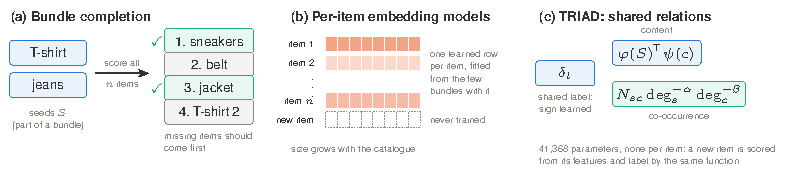
\includegraphics[width=.8\textwidth]{figs/fig1.pdf}
\caption{(a) Bundle completion ranks every catalogue item for a partial bundle. (b) Per-item models such as CLHE and
RaMen store part of their knowledge in one learned row per item. (c) TRIAD learns relations that are shared by all
items: over labels, between item features, and over co-occurrence counts.}
\label{fig:intro}
\end{figure}

% =====================================================================================================================
\section{Related Work}

\paragraph{Bundle construction.} Bundle recommendation ranks existing bundles for a user \cite{bgcn,crosscbr}, and
personalized bundle generation creates one for a user \cite{bgn,pog}. Bundle construction starts from a partial
bundle and has no user. CLHE \cite{clhe}, RaMen \cite{ramen} and Caro \cite{caro} learn item representations from
% [hidden for now: DDBC / Bundle-MLLM] several views and score candidates against a pooled seed vector; Bundle-MLLM \cite{bundlemllm} and in-context
% [hidden for now: DDBC / Bundle-MLLM] prompting \cite{adabundle} use language models; DDBC \cite{ddbc} generates the missing set jointly. Set models such as DeepSets
several views and score candidates against a pooled seed vector, and language models have been prompted to build
bundles \cite{adabundle}. Set models such as DeepSets
\cite{deepsets} and the Set Transformer \cite{settransformer}, and basket completion with determinantal point
processes \cite{gartrell2017}, also pool learned item embeddings; TRIAD pools fixed item statistics and learns functions of
them shared by all items. Feature-based cold-start models \cite{lightfm,dropoutnet} map new items into a per-item latent space;
TRIAD has none, so a new item is scored by the same content and label terms as any other.

\paragraph{Simple item-to-item methods.} ItemKNN \cite{sarwar2001}, RP3$\beta$ \cite{rp3beta}, EASE \cite{steck2019}
and graph filters \cite{gfcf,sgfcf} remain strong in recommendation once tuned \cite{dacrema,rendle2020}; latent-factor
models \cite{hu2008,bpr,lightgcn} learn one embedding per item. How two items relate depends on their categories
\cite{han2017,vasileva2018,mcauley}; TRIAD keeps one label rule per level. Training on statistics that contain the example itself leaks
its answer \cite{kapoor2023}; TRIAD removes each training bundle from its own counts exactly.

% =====================================================================================================================
\section{Method}
\label{sec:method}

\begin{figure}[t]
\centering
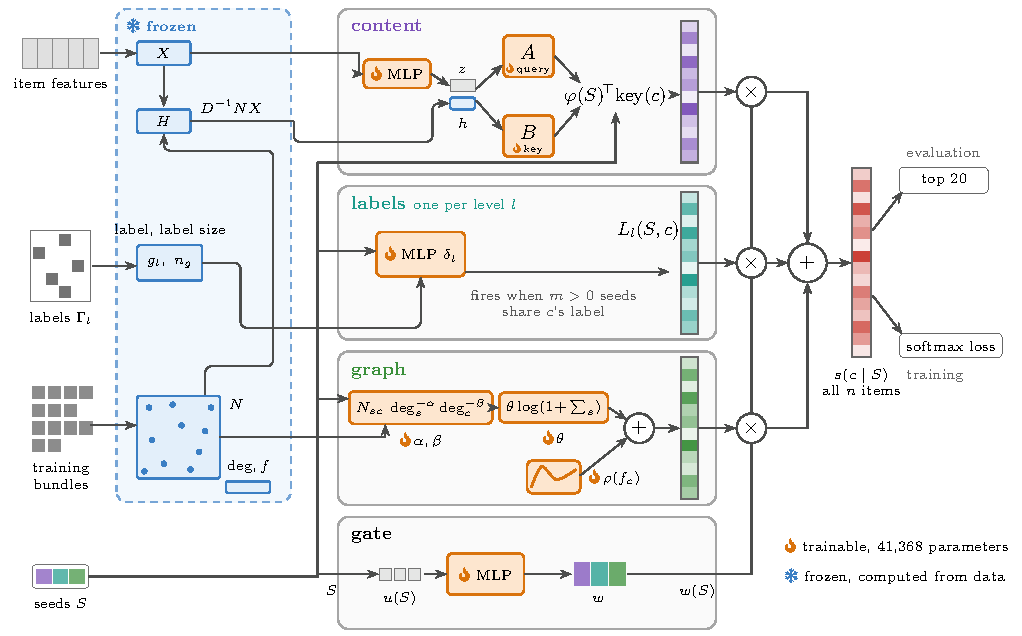
\includegraphics[width=.86\textwidth]{figs/fig2_arch.pdf}
\caption{TRIAD. Frozen structures (blue) are computed once from item features, labels and training bundles. Each term
gives a score vector over all $n$ items; the gate weights them per query. All 41,368 trained parameters (orange) are
shared by all items.}
\label{fig:arch}
\end{figure}

\paragraph{Notation.} The catalogue has $n$ items. Item $c$ has a feature vector $x_c$ (rows of $X\in\R^{n\times d}$,
unit length) and, at each label level $l$, a label $g_l(c)$: the category for fashion and e-commerce, artist and album
for music. From the training bundles $\B$ we count $N_{sc}$, the number of bundles that contain both $s$ and $c$
($s\neq c$), the item frequency $f_c$ and the degree $\deg_c=\sum_s N_{sc}$. A query is a seed set $S$; all items not
in $S$ are ranked.

\paragraph{Features.} POG and Spotify come with released BLIP \cite{blip} image and text embeddings and CLAP
\cite{clap} audio and text embeddings; for e-commerce we embed each title with BLIP's text encoder. The modalities are
row-normalized, concatenated and projected by a rank-128 truncated SVD to $X$ ($d=128$), using no bundle or label. Every
simple content baseline uses exactly this $X$, and CLHE and RaMen the unprojected vectors; we verified both.

\paragraph{Score.} TRIAD scores every item $c$ by asking three questions of it: does it look like it belongs with
the seeds, does it share a label with them, and has it been bundled with them before? The answers are combined by a
gate $w(S)$ that depends on the query (Fig.~\ref{fig:arch}):
\begin{equation}
s(c\mid S)=w_C(S)\,C(S,c)+\textstyle\sum_l w_l(S)\,L_l(S,c)+w_G(S)\,G(S,c).
\label{eq:score}
\end{equation}


\paragraph{Content.} The first question is about appearance and company. Item features are refined by a small
residual network, $Z=\mathrm{normalize}(X+\mathrm{MLP}(X))$, and each item also carries a \emph{partner history}, the
count-weighted mean feature of the items it has been bundled with, $H=\mathrm{diag}(\deg)^{-1}NX$. The history
describes an item by the company it keeps, not only by what it is. Then
\begin{equation}
C(S,c)=\varphi(S)^{\top}\psi(c),\ \ \varphi(S)=\tfrac{1}{|S|}\textstyle\sum_{s\in S}(A_z z_s+A_h h_s),\ \
\psi(c)=B_z z_c+B_h h_c,
\end{equation}
with $A_z,A_h,B_z,B_h\in\R^{64\times d}$. Separate seed-side and candidate-side maps make the relation asymmetric: a
jacket can call for boots without boots calling for a jacket.

\paragraph{Labels.} The second question is whether the candidate shares a label with the seeds, and whether that is
good news. With $m$ the number of seeds that share the candidate's label at level $l$ and $n_g$ the size of label $g$,
\begin{equation}
L_l(S,c)=\deltab_l\big(\log(1+m),\log|S|,\log(1+n_{g_l(c)})\big)\cdot[m>0],
\end{equation}
where $\deltab_l$ is a small MLP shared by all labels of the level. Its output may be negative, so the model can learn
that a shared label counts \emph{against} a candidate, which is exactly what an outfit needs. Which different labels
go together, such as skirts with sandals, is left to the item counts $N$, of which a label-level table would only be
a coarser summary.

\paragraph{Graph.} The third question is whether the candidate has been bundled with the seeds before. Counts are
discounted for items bundled with everything, and a small MLP $\rho$ adds a learned popularity prior:
\begin{equation}
G(S,c)=\theta\log\Big(1+\textstyle\sum_{s\in S}N_{sc}\deg_s^{-\alpha}\deg_c^{-\beta}\Big)+\rho\big(\log(1+f_c)\big).
\end{equation}

\paragraph{Gate.} Finally, the gate decides how much each answer counts. It reads three statistics of the query, its
size $\log|S|$, the mean seed $\log(1+f_s)$ and the share of seeds with $f_s=0$, and returns
$w(S)=\mathrm{softplus}(\mathrm{MLP}(u(S)))$. When none of the seeds has been bundled before there are no counts to
rely on, and the gate can shift weight to content and labels.

\paragraph{Training without leakage.} Each step hides part of 32 training bundles (half of the items with
probability $1/2$, otherwise a uniform cut) and asks TRIAD to recover them from the rest: a hidden item $j$ competes
with every item outside its bundle through the loss $\mathrm{softplus}(\mathrm{LSE}_{c\notin b}\,s(c\mid S)-s(j\mid
S))$. This is where a trap lies. A training bundle $b$ is itself part of $N$, $f$, $\deg$ and $H$, so the counts
between its seeds and its hidden items already contain the answer, a shortcut no test query offers. Each training
bundle is therefore scored with its own contribution removed: $N_{sc}-1$ for pairs inside $b$, $\deg-(|b|-1)$ and
$f-1$ for its members, and the same correction in $H$. Only the seeds' rows change, so the correction costs little.

\paragraph{One configuration.} AdamW \cite{adamw} (learning rate $10^{-2}$ for the relation parameters, $10^{-3}$ for
the content maps and encoder, weight decay $10^{-3}$), early stopping on validation NDCG@20. Initialization makes
training start from plain feature similarity with every term weighted 1 and no degree discount. Nothing is tuned per
dataset, and the e-commerce datasets were not used during development. The 41,368 parameters (41,466 with two label
levels) are 32,768 in the content maps, 8,352 in the encoder and 248--346 in the label score, graph and gate,
independent of $n$.

\paragraph{How TRIAD differs from a tuned blend.} Unlike a simple scorer whose weights are set by grid search,
TRIAD learns (i) how far to trust each signal for each query, through the gate, instead of one weight per dataset;
(ii) the degree discounts, the popularity prior and the sign and strength of the label rule, jointly rather than one
method at a time; and (iii) an asymmetric content relation that also compares the seeds with a candidate's partner
history, so it can score complements, not only look-alikes. Leave-one-out statistics make this trainable on co-occurrence.
Removing the gate costs up to .065 NDCG@20, removing leave-one-out up to .165, and training adds .030 to .179
(Table~\ref{tab:ablation}).

% =====================================================================================================================
\section{Experimental Setup}

\paragraph{Datasets} (Table~\ref{tab:data}). POG and POG\_DENSE are outfits made by Taobao's fashion experts
\cite{pog}, Spotify and Spotify\_sparse playlists made by Spotify users \cite{spotify}, all with the split files
released with CLHE \cite{clhe}, used unchanged. Electronic, Food and Clothing are bundles marked by crowd workers in
Amazon shopping sessions \cite{bundlerec}; we remove duplicate bundles and bundles with fewer than two distinct items,
split 70/10/20 with a fixed seed and hide half of each validation and test bundle.

\begin{table}[t]
\centering
\caption{Datasets. Size: mean items per training bundle. Labels: values per level. Test: queries, clean ones (whose
bundle occurs in neither training nor validation) in brackets.}
\label{tab:data}
\setlength{\tabcolsep}{3pt}
\scriptsize
\begin{tabular}{llrrrrl}
\toprule
Bundles made by & Dataset & Items & Train & Size & Test & Labels\\
\midrule
crowd workers & Electronic & 3,499 & 1,211 & 3.5 & 346 & 479\\
 & Food & 3,767 & 1,232 & 3.5 & 353 & 836\\
 & Clothing & 4,487 & 1,294 & 3.3 & 371 & 2,033\\
fashion experts & POG\_DENSE & 31,217 & 20,780 & 3.6 & 5,938 (5,547) & 67\\
 & POG & 48,676 & 14,000 & 3.6 & 4,000 (3,995) & 72\\
playlist users & Spotify\_sparse & 213,325 & 8,740 & 44.2 & 2,498 (2,497) & 43,039; 98,674\\
 & Spotify & 254,155 & 14,000 & 63.6 & 4,000 (3,995) & 49,164; 116,217\\
\bottomrule
\end{tabular}
\end{table}

\paragraph{Protocol.} Every method ranks the full catalogue with the seeds removed; we report Recall@20 and NDCG@20 on
clean test queries, so that a method cannot score by memorizing a test bundle that also occurs in training. Learned models run with three seeds, and per-query metrics are averaged over them.
Differences come with a 95\% paired bootstrap interval and a paired sign-flip test, both resampling clusters of
identical bundles \cite{efron1993,smucker2007}, with Holm's correction \cite{holm1979} within each table. Ranking the
full catalogue avoids the bias of sampled metrics \cite{krichene2020}.

\paragraph{Baselines.} \emph{Simple:} popularity, co-occurrence, ItemKNN, RP3$\beta$, EASE, GF-CF, SGFCF, iALS, a
blend of ItemKNN with content cosine, and four label-aware methods (same-label counts, label transitions, and the
better of the two blended with ItemKNN, with and without content). Each gets a validation grid (1 to 24 settings, more with the prior), and
the best method per dataset is chosen on validation. \emph{Neural:} CLHE and RaMen, rerun as released with settings
chosen on validation (the best of CLHE's four released settings and 10 RaMen settings on e-commerce), with user and
item graphs from training bundles only. RaMen's item--item graph is not released, so we built it as its paper
describes. We quote RaMen's published numbers on POG and Spotify (same split files); on full Spotify only one CLHE seed
finished within 12 hours, so it is not tested there. TRIAD uses one configuration everywhere.

\paragraph{Equal information.} One property of these benchmarks shapes every comparison, so we describe it before the
results. The released catalogues hold exactly the items that occur in some training, validation or test bundle. The
19--25\% of items that occur in no training bundle ($f=0$) are therefore all items of validation or test bundles, and
they are likely targets: $f=0$ for 41--67\% of e-commerce test targets, 23\% on POG\_DENSE, 59\% on POG, 29\% on
Spotify\_sparse and 14\% on Spotify. No test answer is involved, but a model trained against the full catalogue can
learn the pattern, and TRIAD does so from training data alone: under leave-one-out, a training target seen in no other
training bundle has $f=0$, and the base-rate gap this produces is within .25 of the test gap on every dataset. Frequency-based baselines, by contrast, rank
$f=0$ items last \cite{abdollahpouri2017}. To compare fairly, we give the five main simple baselines (ItemKNN,
RP3$\beta$, EASE, content+ItemKNN, label+ItemKNN+content) the same prior, $\lambda\,b(f_c)$ added to the max-scaled
score with $b$ the base rate of validation targets by frequency and $\lambda\in\{0,.01,\dots,3\}$ chosen on
validation, and report TRIAD without this
unseen-item bonus ($\rho$ of $f=0$ items set to its value at $f=1$).

% =====================================================================================================================
\section{Results}

\begin{table}[t]
\centering
\caption{Recall@20 (R) and NDCG@20 (N) on clean test queries (learned models: mean of three seeds). Simple baselines may
use the frequency prior ($\lambda$ chosen on validation). Bold: best, TRIAD w/o bonus excluded. Last row: trained
parameters of CLHE / RaMen (TRIAD: 41\,k). $^\dagger$Published, all test queries. $^\ddagger$One of three seeds, all
test queries.}
\label{tab:main}
\setlength{\tabcolsep}{3.2pt}
\scriptsize
\begin{tabular}{lcccccc}
\toprule
 & \multicolumn{2}{c}{Electronic} & \multicolumn{2}{c}{Food} & \multicolumn{2}{c}{Clothing}\\
\cmidrule(lr){2-3}\cmidrule(lr){4-5}\cmidrule(lr){6-7}
Method & R & N & R & N & R & N\\
\midrule
ItemKNN & .352 & .248 & .338 & .262 & .238 & .194\\
RP3$\beta$ & .353 & .255 & .342 & .275 & .238 & .195\\
EASE & .354 & .254 & .342 & .267 & .238 & .201\\
Content+ItemKNN & .435 & .312 & .583 & .460 & .582 & .427\\
Label+ItemKNN+content & .437 & .320 & .594 & .464 & \textbf{.594} & \textbf{.440}\\
\midrule
CLHE & .362 & .259 & .419 & .271 & .325 & .196\\
RaMen & .345 & .256 & .345 & .265 & .240 & .190\\
\midrule
TRIAD & \textbf{.467} & \textbf{.335} & \textbf{.618} & \textbf{.474} & .593 & .439\\
\emph{TRIAD w/o bonus} & .405 & .306 & .581 & .445 & .485 & .355\\
\midrule
Parameters & \multicolumn{2}{c}{3.7\,M / 1.3\,M} & \multicolumn{2}{c}{3.7\,M / 1.4\,M} & \multicolumn{2}{c}{3.8\,M / 1.6\,M}\\
\bottomrule
\end{tabular}

\medskip
\begin{tabular}{lcccccccc}
\toprule
 & \multicolumn{2}{c}{POG\_DENSE} & \multicolumn{2}{c}{POG} & \multicolumn{2}{c}{Spotify\_sparse} & \multicolumn{2}{c}{Spotify}\\
\cmidrule(lr){2-3}\cmidrule(lr){4-5}\cmidrule(lr){6-7}\cmidrule(lr){8-9}
Method & R & N & R & N & R & N & R & N\\
\midrule
ItemKNN & .340 & .232 & .029 & .019 & .116 & .149 & .130 & .219\\
RP3$\beta$ & .345 & .241 & .030 & .020 & .118 & .149 & .124 & .210\\
EASE & .333 & .237 & .029 & .019 & -- & -- & -- & --\\
Content+ItemKNN & .340 & .232 & .029 & .019 & .120 & .155 & .133 & .223\\
Label+ItemKNN+content & .342 & .249 & .036 & .023 & .151 & .209 & .147 & .247\\
\midrule
CLHE & .349 & .248 & .026 & .017 & .097 & .115 & .108 & .179$^\ddagger$\\
RaMen & -- & -- & .037 & .023$^\dagger$ & -- & -- & .109 & .188$^\dagger$\\
\midrule
TRIAD & \textbf{.374} & \textbf{.278} & \textbf{.052} & \textbf{.031} & \textbf{.184} & \textbf{.256} & \textbf{.167} & \textbf{.282}\\
\emph{TRIAD w/o bonus} & .374 & .278 & .048 & .029 & .183 & .255 & .167 & .282\\
\midrule
Parameters & \multicolumn{2}{c}{7.2\,M / 11.6\,M} & \multicolumn{2}{c}{9.5\,M / 16.1\,M} & \multicolumn{2}{c}{29\,M / 56.5\,M} & \multicolumn{2}{c}{-- / 67\,M}\\
\bottomrule
\end{tabular}
\end{table}

\begin{table}[t]
\centering
\caption{TRIAD minus the best simple baseline (chosen on validation over all thirteen; $^{*}$: with the prior), clean
test queries: $\Delta$ NDCG@20 with 95\% cluster-bootstrap interval and Holm-corrected sign-flip $p$ over 14 tests
(bold: $p<.05$).}
\label{tab:tests}
\setlength{\tabcolsep}{1.6pt}
\scriptsize
\begin{tabular}{lllrrlr}
\toprule
& & \multicolumn{3}{c}{TRIAD $-$ best simple} & \multicolumn{2}{c}{w/o bonus $-$ best simple}\\
\cmidrule(lr){3-5}\cmidrule(lr){6-7}
Dataset & Best simple & $\Delta$ N@20 [95\% CI] & $p$ (N) & $p$ (R) & $\Delta$ N@20 [95\% CI] & $p$ (N)\\
\midrule
Electronic & content+kNN$^{*}$ & +.022 [.004, .042] & .116 & .116 & $-$.006 [$-$.025, .013] & 1.000\\
Food & content+kNN$^{*}$ & +.014 [$-$.003, .031] & .373 & \textbf{.026} & $-$.015 [$-$.031, .001] & .198\\
Clothing & content+kNN$^{*}$ & +.011 [$-$.005, .027] & .373 & .383 & $-$.072 [$-$.094, $-$.052] & \textbf{.001}\\
POG\_DENSE & RP3$\beta$ & +.037 [.034, .041] & \textbf{.001} & \textbf{.001} & +.037 [.034, .041] & \textbf{.001}\\
POG & lab.+kNN+cont. & +.007 [.005, .009] & \textbf{.001} & \textbf{.001} & +.005 [.004, .007] & \textbf{.001}\\
Spotify\_sparse & lab.+kNN+cont.$^{*}$ & +.048 [.043, .052] & \textbf{.001} & \textbf{.001} & +.047 [.042, .051] & \textbf{.001}\\
Spotify & lab.+kNN+cont. & +.035 [.031, .040] & \textbf{.001} & \textbf{.001} & +.035 [.031, .040] & \textbf{.001}\\
\bottomrule
\end{tabular}

\end{table}

\paragraph{Outfits and playlists: TRIAD is ahead.} On outfits and playlists TRIAD is ahead of the best simple baseline on every dataset
(Tables~\ref{tab:main},~\ref{tab:tests}), and all eight tests agree after Holm correction. The margins are largest on the playlists (+.048 and +.035 NDCG@20)
and smallest on POG (+.007), where every method struggles. Removing the unseen-item bonus hardly moves them, so these
leads come from the relations themselves.

\paragraph{E-commerce: level with a simple baseline that has the same information.} The short e-commerce bundles
tell a different story. TRIAD's average lead over the content+ItemKNN blend is still positive (+.022, +.014, +.011
NDCG@20), but only Food's Recall@20 difference survives Holm, and on Clothing the label-aware blend edges ahead (.440
against .439). Without the bonus TRIAD falls behind on all three, clearly so on Clothing ($-$.072). On these short
bundles, most of TRIAD's lead comes from how it treats items that no training bundle contains.

\paragraph{Neural models trail TRIAD and, mostly, simple methods.} Against the neural models the picture is
unambiguous. TRIAD is ahead of CLHE on all six datasets where we reran it (+.013 to +.242 NDCG@20) and of RaMen on all
three e-commerce sets (+.078 to +.249); all nine differences and their Recall@20 counterparts hold after Holm. More
telling is that the tuned simple baselines already match or beat CLHE in NDCG@20 everywhere (on POG\_DENSE .249
against .248) and beat RaMen on e-commerce by .06--.25. RaMen's own e-commerce numbers are another matter. It reports Recall@20 of .837 and .846 on Electronic and
Food, on a split that is not released. The data include a user--item file that holds the items of every bundle, test
bundles included, and RaMen rerun on our split with a graph built from it reaches .505 / .490 / .499 instead of
.345 / .345 / .240.

\paragraph{The bonus follows the catalogue, not the split.} Is the unseen-item bonus a quirk of our split or of the
benchmarks? On Electronic and Food we retrained TRIAD on two fresh random splits and on the published split padded
with $P=1$, 4 and 16 times $n_0$ never-bundled items ($n_0$: items with $f=0$), each a copy of a random item's
features and category. A new split changes nothing: the learned bonus stays at 1.4--1.9, still adds .017--.042
NDCG@20 (all significant), and TRIAD stays level with the best simple baseline (+.011 to +.025, none significant;
Holm over 48 tests). Padding the catalogue removes the effect. As never-bundled items become common, the learned bonus
shrinks from training data alone, following the base rate the test calls for, and turns into a penalty at $16n_0$;
its gain falls from .028 and .029 to .007 and .013 at $P=n_0$ and to zero from $4n_0$, while TRIAD stays level with
the best simple baseline ($-$.009 to +.014, none significant). The advantage comes from how the benchmarks are built.

% [hidden for now: DDBC / Bundle-MLLM] \begin{table}[t]
% [hidden for now: DDBC / Bundle-MLLM] \centering
% [hidden for now: DDBC / Bundle-MLLM] \caption{Under other papers' protocols, without retraining. Top: HitRate@1 among 10 candidates (Bundle-MLLM's protocol);
% [hidden for now: DDBC / Bundle-MLLM] every question (POG) or 8,192 sampled ones (Spotify, at most 5 seeds shown, as Bundle-MLLM does), three seeds $\times$
% [hidden for now: DDBC / Bundle-MLLM] five draws. Bundle-MLLM and CLHE: published in Bundle-MLLM's paper (2,048 questions). Simple: the best simple baseline
% [hidden for now: DDBC / Bundle-MLLM] of Table~\ref{tab:tests} on the same questions. Bottom: F1 / Jaccard under DDBC's pool protocol; DDBC rerun from its
% [hidden for now: DDBC / Bundle-MLLM] released checkpoints on the same pools; simple: best on validation, without the prior (RP3$\beta$ on POG\_DENSE, the content+ItemKNN
% [hidden for now: DDBC / Bundle-MLLM] blend on Spotify); DDBC's best baseline as published (TIGER, BundleNAT at $k{=}30$). Paired tests TRIAD $-$ simple (HitRate@1, Holm over 4) and TRIAD $-$ DDBC (Holm over 8): all $p<.001$.}
% [hidden for now: DDBC / Bundle-MLLM] \label{tab:protocols}
% [hidden for now: DDBC / Bundle-MLLM] \setlength{\tabcolsep}{3pt}
% [hidden for now: DDBC / Bundle-MLLM] \scriptsize
% [hidden for now: DDBC / Bundle-MLLM] \begin{tabular}{lccccc}
% [hidden for now: DDBC / Bundle-MLLM] \toprule
% [hidden for now: DDBC / Bundle-MLLM] HitRate@1 & TRIAD & w/o bonus & Simple & Bundle-MLLM & CLHE\\
% [hidden for now: DDBC / Bundle-MLLM] \midrule
% [hidden for now: DDBC / Bundle-MLLM] POG\_DENSE & \textbf{.771} & .743 & .617 & .668 & .637\\
% [hidden for now: DDBC / Bundle-MLLM] POG & \textbf{.624} & .513 & .306 & .413 & .348\\
% [hidden for now: DDBC / Bundle-MLLM] Spotify\_sparse & \textbf{.814} & .816 & .641 & .796 & .723\\
% [hidden for now: DDBC / Bundle-MLLM] Spotify & \textbf{.841} & .841 & .759 & .824 & .757\\
% [hidden for now: DDBC / Bundle-MLLM] \bottomrule
% [hidden for now: DDBC / Bundle-MLLM] \end{tabular}
%
% [hidden for now: DDBC / Bundle-MLLM] \medskip
% [hidden for now: DDBC / Bundle-MLLM] \begin{tabular}{lccccc}
% [hidden for now: DDBC / Bundle-MLLM] \toprule
% [hidden for now: DDBC / Bundle-MLLM] F1 / Jaccard & TRIAD & w/o bonus & Simple & DDBC (rerun) & DDBC's best\\
% [hidden for now: DDBC / Bundle-MLLM] \midrule
% [hidden for now: DDBC / Bundle-MLLM] POG\_DENSE $k{=}4$ & \textbf{.483 / .392} & .482 / .391 & .452 / .360 & .138 / .099 & .213 / .157\\
% [hidden for now: DDBC / Bundle-MLLM] Spotify $k{=}30$ & \textbf{.625 / .482} & .625 / .482 & .544 / .406 & .279 / .176 & .153 / .090\\
% [hidden for now: DDBC / Bundle-MLLM] Spotify $k{=}60$ & \textbf{.643 / .495} & .643 / .495 & .562 / .416 & .285 / .178 & .129 / .076\\
% [hidden for now: DDBC / Bundle-MLLM] Spotify $k{=}90$ & \textbf{.651 / .501} & .651 / .501 & .564 / .415 & .278 / .171 & .123 / .070\\
% [hidden for now: DDBC / Bundle-MLLM] \bottomrule
% [hidden for now: DDBC / Bundle-MLLM] \end{tabular}
% [hidden for now: DDBC / Bundle-MLLM] \end{table}
%
% [hidden for now: DDBC / Bundle-MLLM] \paragraph{Bundle-MLLM's and DDBC's protocols.} The two remaining models report results under their own protocols,
% [hidden for now: DDBC / Bundle-MLLM] both on CLHE's split files with sampled candidates (Table~\ref{tab:protocols}). \emph{Bundle-MLLM} asks which of ten
% [hidden for now: DDBC / Bundle-MLLM] candidates (a held-out item and nine random ones) belongs. Its released checkpoints cannot be run with the inputs
% [hidden for now: DDBC / Bundle-MLLM] they were trained on: its prompts use English item titles
% [hidden for now: DDBC / Bundle-MLLM] that are not released, and it uses BLIP2 image features released only for POG. Against its published numbers TRIAD
% [hidden for now: DDBC / Bundle-MLLM] is ahead by .10--.21 on the two outfit datasets and by .017 and .018 on the playlists; at about two standard
% [hidden for now: DDBC / Bundle-MLLM] errors of its 2,048-question estimate, we do not claim the latter. Here, unlike elsewhere, the
% [hidden for now: DDBC / Bundle-MLLM] tuned simple methods fall \emph{below} the published model, by .05--.16, while TRIAD stays ahead of them by .08--.32
% [hidden for now: DDBC / Bundle-MLLM] on the same questions (all $p<.001$). \emph{DDBC} splits windows of our test bundles into seed and target halves and
% [hidden for now: DDBC / Bundle-MLLM] ranks the targets among 99 random items each. Its released checkpoints reproduce its published F1 (.137--.278 against
% [hidden for now: DDBC / Bundle-MLLM] .139--.287), yet a tuned simple method reaches about three times that F1 on POG\_DENSE and twice on Spotify, and
% [hidden for now: DDBC / Bundle-MLLM] TRIAD is higher still. The unseen-item bonus changes F1 by at most .001 here.

\begin{figure}[t]
\centering
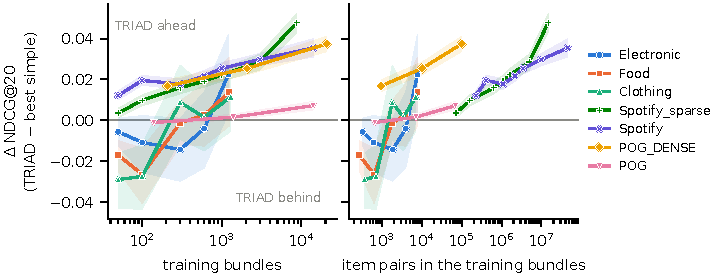
\includegraphics[width=.84\textwidth]{figs/fig3_budget.pdf}
\caption{TRIAD minus the best simple baseline (with the prior allowed, chosen on validation for every subset), NDCG@20
on clean test with 95\% interval, against the number of training bundles (left) and of item pairs they contain
(right).}
\label{fig:budget}
\end{figure}

\begin{table}[t]
\centering
\caption{Ablations: NDCG@20 of the full model minus the ablated model (clean test, three seeds per side). Bold: Holm
$p<.05$ over 12 tests per row. First row: NDCG@20 of the full model.}
\label{tab:ablation}
\setlength{\tabcolsep}{3pt}
\scriptsize
\begin{tabular}{lcccccc}
\toprule
Removed part & Electronic & Food & Clothing & POG\_DENSE & POG & Spotify\_sparse\\
\midrule
\emph{full model (NDCG@20)} & .335 & .474 & .439 & .278 & .031 & .256\\
\midrule
leave-one-out statistics & \textbf{.054} & \textbf{.140} & \textbf{.165} & \textbf{.073} & \textbf{.010} & \textbf{.112}\\
gate (all weights 1) & \textbf{.065} & \textbf{.036} & \textbf{.031} & \textbf{.002} & .001 & \textbf{.008}\\
content term & \textbf{.046} & \textbf{.125} & \textbf{.153} & \textbf{.031} & \textbf{.010} & \textbf{.016}\\
label terms & .002 & .002 & .009 & \textbf{.003} & \textbf{.002} & \textbf{.088}\\
graph term & \textbf{.185} & \textbf{.172} & \textbf{.152} & \textbf{.014} & \textbf{.019} & \textbf{.059}\\
training (initial parameters) & \textbf{.159} & \textbf{.129} & \textbf{.179} & \textbf{.177} & \textbf{.030} & \textbf{.117}\\
\bottomrule
\end{tabular}
\end{table}

\paragraph{Which parts carry the weight?} Removing co-occurrence, leave-one-out training or the content term hurts
on all six datasets (Table~\ref{tab:ablation}; full Spotify omitted, 1--1.5\,h of CPU per run). Leave-one-out matters
for the reason given in Section~\ref{sec:method}: without it the model learns to read the answer from a bundle's own
counts, its training loss collapses (2.6 against 6.5 on POG\_DENSE), and its test accuracy falls on every dataset. The
gate matters most on the small e-commerce catalogues, the label terms on playlists.


\paragraph{How much training data?} We retrain TRIAD, and retune ten simple baselines with the prior, on nested
random subsets of the training bundles, keeping validation and test fixed (Fig.~\ref{fig:budget}; Holm within each
domain). The answer depends on the domain. On playlists TRIAD stays ahead all the way down to 50 bundles (+.012 and
+.004 NDCG@20; all 28 tests significant). On POG\_DENSE it keeps its lead with 10\% and 1\% of the outfits (+.025,
+.017), while on POG every method scores below .004 at 1\%. On
e-commerce it is never significantly ahead from the full 1,200--1,300 bundles down to 300, and with 100 or 50
bundles it falls behind by .006--.029, significantly on Food and Clothing. The cause is overfitting rather than too
few updates: matching the full data's number of gradient steps changes test NDCG@20 by at most .02.

\paragraph{What TRIAD learns.} Because every trained part is a function of a few interpretable inputs, we can read
what TRIAD has learned. The clearest case is the label rule. $\deltab_l$ starts with no fixed sign, and training gives
it the sign of the domain: strongly negative on outfits ($-$22.5 on POG\_DENSE and $-$6.17 on POG, for one shared
seed at the median label size), so a candidate in a seed's category is pushed out of the shortlist; positive on
playlists (+1.88 for a shared artist and +1.17 for a shared album on Spotify\_sparse); and mildly positive on
e-commerce. Nobody told the model that outfits avoid repeated categories or that playlists revisit artists; it found
both in the bundles. The gate behaves as intended too: as the share of unseen seeds goes from 0 to 1, its weight on
content rises on every dataset, by 18--64\%.

% =====================================================================================================================
\section{Conclusion}

Bundle completion does not need a learned representation per item. Learning how to weigh relations that every item
shares (content, labels and co-occurrence) with 41,368 parameters and training statistics that never contain the
% [hidden for now: DDBC / Bundle-MLLM] answer is enough to score above CLHE, RaMen, DDBC and Bundle-MLLM. Two lessons reach beyond TRIAD. First, simple
% [hidden for now: DDBC / Bundle-MLLM] methods deserve a place in every comparison: tuned, they match or beat three of these four models. Second, how a benchmark
answer is enough to score above CLHE and RaMen. Two lessons reach beyond TRIAD. First, simple methods deserve a place
in every comparison: tuned, they match or beat both models. Second, how a benchmark
is built can look like modelling progress: on the small e-commerce sets, much of any gain comes from a
catalogue that lists only bundled items. Where bundles carry real structure, in outfits and playlists, a model of shared
relations goes clearly beyond the simple methods; where data are few and bundles short, it does not yet.

\paragraph{Limitations.} On e-commerce TRIAD is not significantly ahead of a simple scorer with the same prior, and it
falls behind with 100 or fewer bundles. The unseen-item bonus is a property of catalogues that hold only bundled
% [hidden for now: DDBC / Bundle-MLLM] items; we checked its removal with copied items, not on a real store catalogue. Bundle-MLLM could not be rerun, and
% [hidden for now: DDBC / Bundle-MLLM] RaMen on POG and Spotify and CLHE on full Spotify are published or single-seed numbers.
items; we checked its removal with copied items, not on a real store catalogue. RaMen on POG and Spotify and CLHE on
full Spotify are published or single-seed numbers. Code will be released.

\begin{thebibliography}{99}\scriptsize
\bibitem{abdollahpouri2017} Abdollahpouri, H., Burke, R., Mobasher, B.: Controlling popularity bias in learning-to-rank recommendation. In: RecSys (2017)
\bibitem{bgn} Bai, J., Zhou, C., Song, J., Qu, X., An, W., Li, Z., Gao, J.: Personalized bundle list recommendation. In: WWW (2019)
\bibitem{bgcn} Chang, J., Gao, C., He, X., Jin, D., Li, Y.: Bundle recommendation with graph convolutional networks. In: SIGIR (2020)
\bibitem{spotify} Chen, C.W., Lamere, P., Schedl, M., Zamani, H.: RecSys Challenge 2018: Automatic music playlist continuation. In: RecSys (2018)
\bibitem{pog} Chen, W., et al.: POG: Personalized outfit generation for fashion recommendation at Alibaba iFashion. In: KDD (2019)
\bibitem{efron1993} Efron, B., Tibshirani, R.J.: An Introduction to the Bootstrap. Chapman \& Hall (1993)
\bibitem{dacrema} Ferrari Dacrema, M., Cremonesi, P., Jannach, D.: Are we really making much progress? A worrying analysis of recent neural recommendation approaches. In: RecSys (2019)
\bibitem{gartrell2017} Gartrell, M., Paquet, U., Koenigstein, N.: Low-rank factorization of determinantal point processes. In: AAAI (2017)
\bibitem{han2017} Han, X., Wu, Z., Jiang, Y.G., Davis, L.S.: Learning fashion compatibility with bidirectional LSTMs. In: ACM MM (2017)
\bibitem{lightgcn} He, X., Deng, K., Wang, X., Li, Y., Zhang, Y., Wang, M.: LightGCN: Simplifying and powering graph convolution network for recommendation. In: SIGIR (2020)
\bibitem{holm1979} Holm, S.: A simple sequentially rejective multiple test procedure. Scandinavian Journal of Statistics 6(2), 65--70 (1979)
\bibitem{hu2008} Hu, Y., Koren, Y., Volinsky, C.: Collaborative filtering for implicit feedback datasets. In: ICDM (2008)
\bibitem{kapoor2023} Kapoor, S., Narayanan, A.: Leakage and the reproducibility crisis in machine-learning-based science. Patterns 4(9) (2023)
\bibitem{krichene2020} Krichene, W., Rendle, S.: On sampled metrics for item recommendation. In: KDD (2020)
\bibitem{lightfm} Kula, M.: Metadata embeddings for user and item cold-start recommendations. In: CBRecSys Workshop at RecSys (2015)
\bibitem{settransformer} Lee, J., Lee, Y., Kim, J., Kosiorek, A., Choi, S., Teh, Y.W.: Set Transformer: A framework for attention-based permutation-invariant neural networks. In: ICML (2019)
\bibitem{blip} Li, J., Li, D., Xiong, C., Hoi, S.: BLIP: Bootstrapping language-image pre-training for unified vision-language understanding and generation. In: ICML (2022)
% [hidden for now: DDBC / Bundle-MLLM] \bibitem{bundlemllm} Liu, X., Wu, J., Tao, Z., Ma, Y., Wei, Y., Chua, T.S.: Fine-tuning multimodal large language models for product bundling. In: KDD (2025)
\bibitem{adamw} Loshchilov, I., Hutter, F.: Decoupled weight decay regularization. In: ICLR (2019)
\bibitem{crosscbr} Ma, Y., He, Y., Zhang, A., Wang, X., Chua, T.S.: CrossCBR: Cross-view contrastive learning for bundle recommendation. In: KDD (2022)
\bibitem{clhe} Ma, Y., Liu, X., Wei, Y., Tao, Z., Wang, X., Chua, T.S.: Leveraging multimodal features and item-level user feedback for bundle construction. In: WSDM (2024)
\bibitem{mcauley} McAuley, J., Pandey, R., Leskovec, J.: Inferring networks of substitutable and complementary products. In: KDD (2015)
\bibitem{ramen} Nguyen, H.S., Nguyen, Q.H., Pham, D.H., Le, D.T., Le, H.Q., Sitkrongwong, P., Takasu, A., Mansoury, M.: RaMen: Multi-strategy multi-modal learning for bundle construction. In: ECAI (2025)
\bibitem{caro} Nguyen, L.H., Nguyen, H.S., Nguyen, C.V.T., Le, D.T., Takasu, A., Le, H.Q.: Dual-enhanced item representation for bundle construction via category-wise and cross-modality learning. In: SIGIR-AP (2025)
\bibitem{rp3beta} Paudel, B., Christoffel, F., Newell, C., Bernstein, A.: Updatable, accurate, diverse, and scalable recommendations for interactive applications. ACM TiiS 7(1) (2017)
\bibitem{sgfcf} Peng, S., Liu, X., Sugiyama, K., Mine, T.: How powerful is graph filtering for recommendation. In: KDD (2024)
\bibitem{bpr} Rendle, S., Freudenthaler, C., Gantner, Z., Schmidt-Thieme, L.: BPR: Bayesian personalized ranking from implicit feedback. In: UAI (2009)
\bibitem{rendle2020} Rendle, S., Krichene, W., Zhang, L., Anderson, J.: Neural collaborative filtering vs. matrix factorization revisited. In: RecSys (2020)
\bibitem{sarwar2001} Sarwar, B., Karypis, G., Konstan, J., Riedl, J.: Item-based collaborative filtering recommendation algorithms. In: WWW (2001)
\bibitem{gfcf} Shen, Y., Wu, Y., Zhang, Y., Shan, C., Zhang, J., Letaief, K.B., Li, D.: How powerful is graph convolution for recommendation? In: CIKM (2021)
\bibitem{smucker2007} Smucker, M.D., Allan, J., Carterette, B.: A comparison of statistical significance tests for information retrieval evaluation. In: CIKM (2007)
\bibitem{steck2019} Steck, H.: Embarrassingly shallow autoencoders for sparse data. In: WWW (2019)
\bibitem{bundlerec} Sun, Z., Feng, K., Yang, J., Fang, H., Qu, X., Ong, Y.S., Liu, W.: Revisiting bundle recommendation for intent-aware product bundling. ACM TORS 2(3) (2024)
\bibitem{adabundle} Sun, Z., Feng, K., Yang, J., Qu, X., Fang, H., Ong, Y.S., Liu, W.: Adaptive in-context learning with large language models for bundle generation. In: SIGIR (2024)
% [hidden for now: DDBC / Bundle-MLLM] \bibitem{ddbc} Tu, T., Li, A., Ma, Y., Xu, S., Liu, X., Ma, H., Pang, L., Chua, T.S.: Discrete diffusion for bundle construction. In: ICLR (2026)
\bibitem{vasileva2018} Vasileva, M.I., Plummer, B.A., Dusad, K., Rajpal, S., Kumar, R., Forsyth, D.: Learning type-aware embeddings for fashion compatibility. In: ECCV (2018)
\bibitem{dropoutnet} Volkovs, M., Yu, G., Poutanen, T.: DropoutNet: Addressing cold start in recommender systems. In: NeurIPS (2017)
\bibitem{clap} Wu, Y., Chen, K., Zhang, T., Hui, Y., Berg-Kirkpatrick, T., Dubnov, S.: Large-scale contrastive language-audio pretraining with feature fusion and keyword-to-caption augmentation. In: ICASSP (2023)
\bibitem{deepsets} Zaheer, M., Kottur, S., Ravanbakhsh, S., Poczos, B., Salakhutdinov, R., Smola, A.: Deep sets. In: NeurIPS (2017)
\end{thebibliography}
\end{document}
